
\subsection{FL Basics}

\begin{figure}[h]
    \centering
    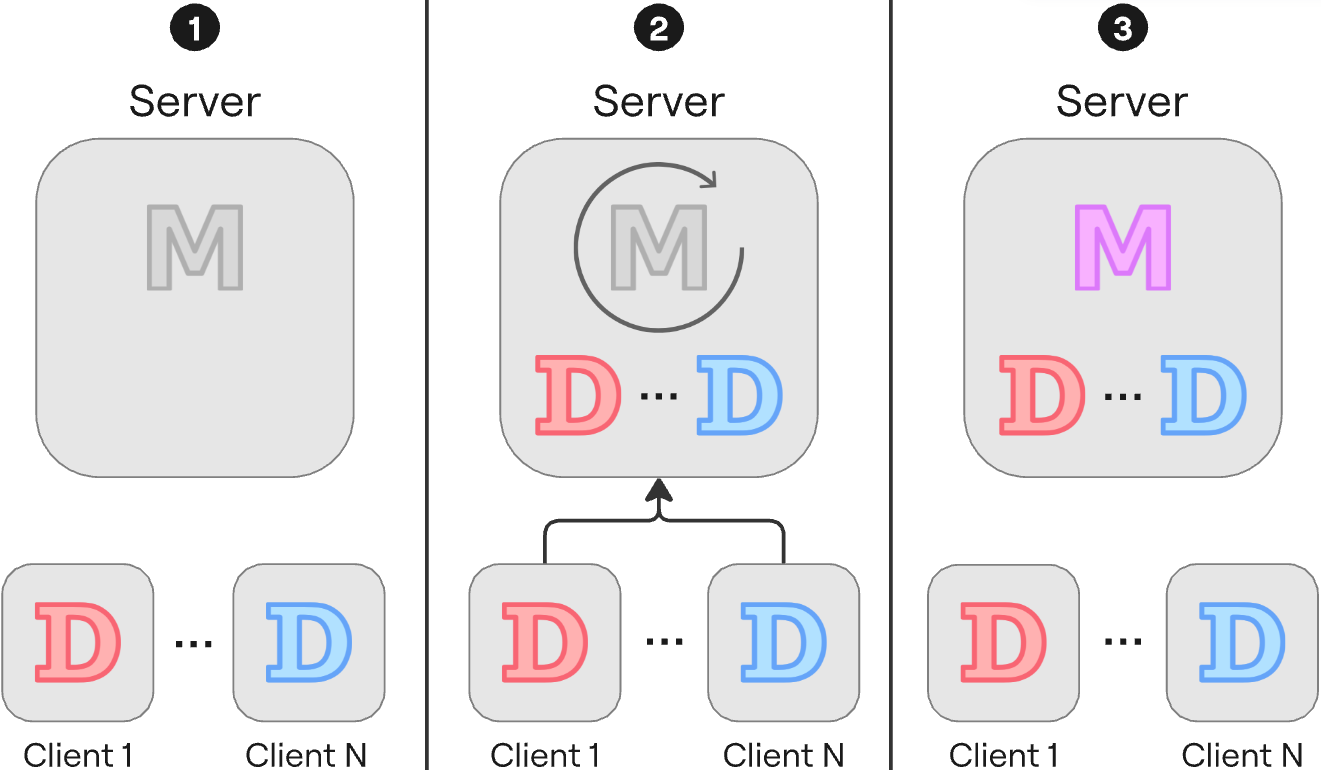
\includegraphics[width=0.9\textwidth]{classic_ml_training.png}
    \caption{Centralized ML Model Training}
    \label{fig:classic_ml_training}
\end{figure}
Figure \ref{fig:classic_ml_training} depicts the classic centralized ML model training process.
Starting from (1), where clients have their data (D) and the server hosts the untrained (gray) ML model (M).
In (2), the clients send their data to the server.
The server can now train the model using data from the clients.
(3) depicts the final state after training.
(The pink/purple model color symbolizes that different data sources have been used during training.)
The client data remains on the server and is exposed to potential exploitation.
As discussed in the introductory chapter, this centralized approach often leads to privacy breaches.

FL was introduced to use sensitive data on client devices for training ML models while keeping that data private.
Thus, FL complies with laws and regulations.
Many different algorithms and strategies exist for FL.
The following example focuses on the widely used base-case/classic FL algorithm FederatedAveraging (FedAvg) \cite{paper:original_fl}.

\begin{figure}%[h]
    \centering
    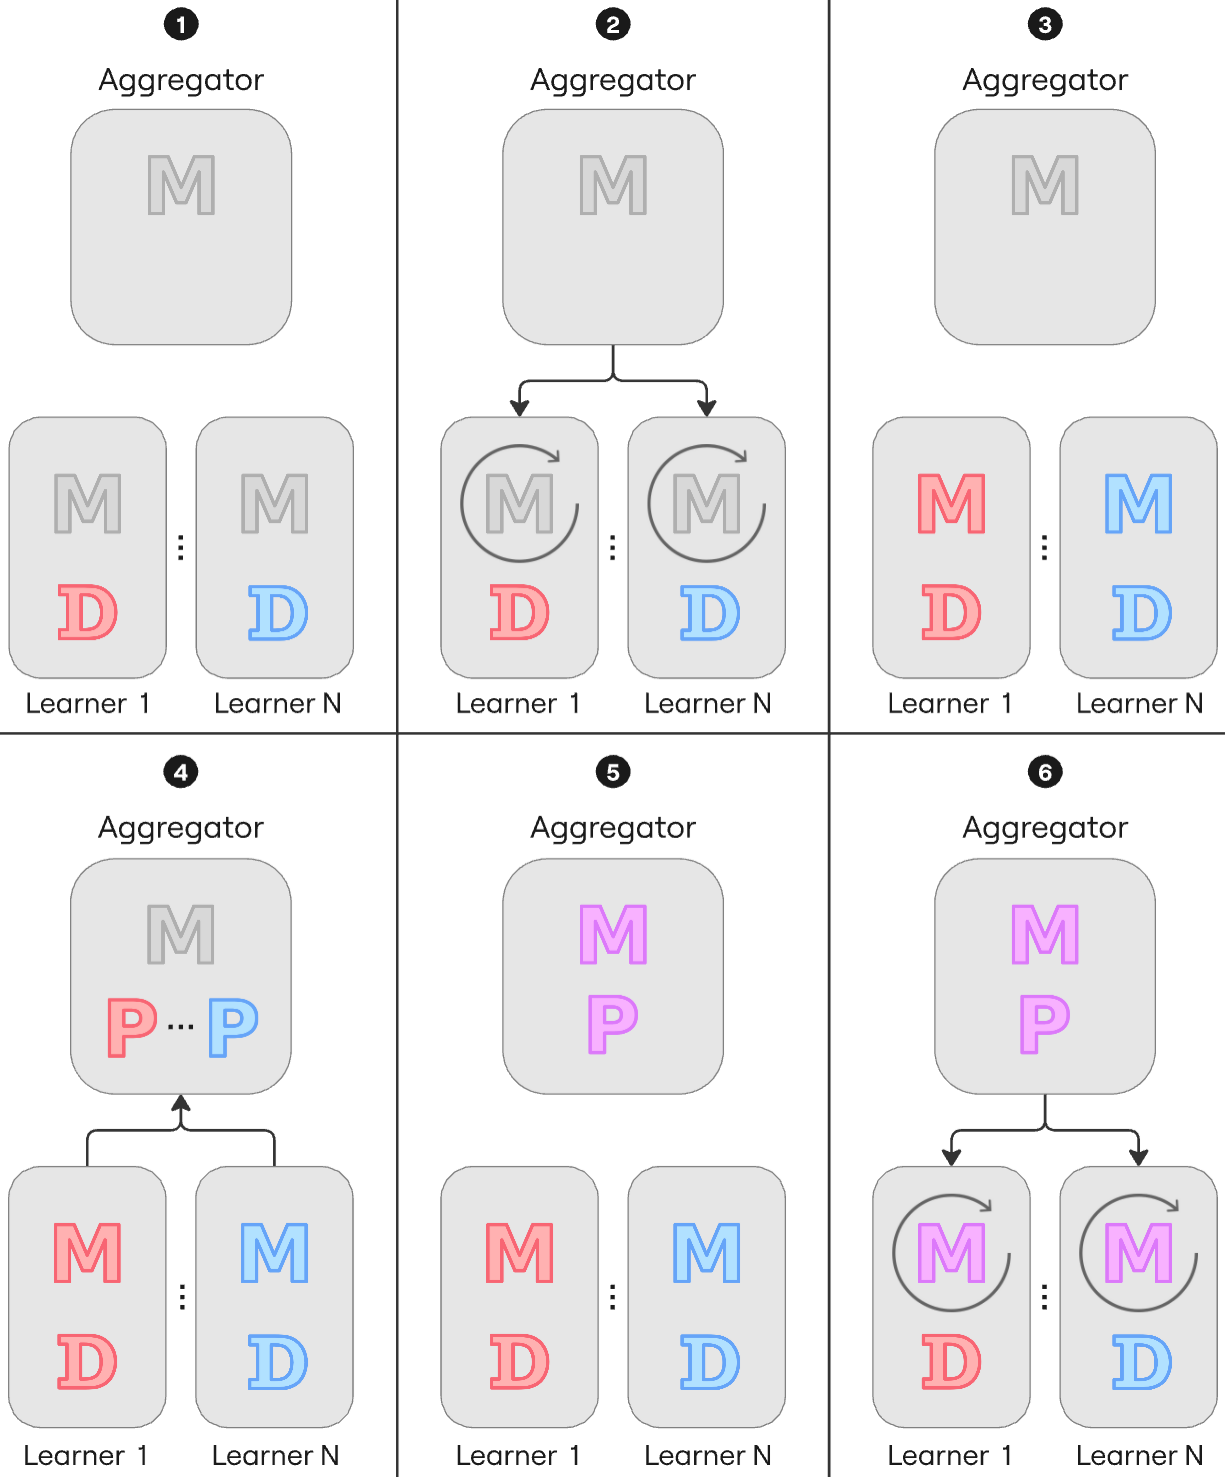
\includegraphics[width=\textwidth]{basic_fl_intro.png}
    \caption{Basic Federated Learning}
    \label{fig:basic_fl_intro}
\end{figure}
Figure \ref{fig:basic_fl_intro} shows the basic FL training loop.
The number of learners can vary.
The first differences are the component names.
In FL, the server is frequently called an \textbf{aggregator}, and it coordinates the FL processes.
Clients are called \textbf{learners}.
Using the terms server and clients in FL is still common
\footnote{
FLOps uses various components, including non-FL servers and clients.
Therefore, this work prefers aggregators and learners because they highlight FL components and help with comprehension.
}.
Another difference is that all components must know and possess the ML model locally.
They also need to set up their environment for training properly.

As a reminder, one can split up ML models into two parts.
One part is (usually) a static lightweight model architecture.
It includes layer specification (in DNNs), training configuration, and hyperparameters like learning step sizes, loss, and activation functions.
Model weights and biases are the dynamic components of an ML model.
A model without them is not useful because weights and biases are what get trained.
They allow the model to fulfill its intended use, such as prediction, inference, or generation tasks.
These weights and biases are the major contributors to a trained model's overall size (space utilization).
Model architecture is static in classic ML/FL.
Thus, FL components can transmit and share weights and biases instead of the entire trained model.
This work calls model relevant data sent between the learners and aggregators (model) \textbf{parameters} and depicts it with (P).

The concrete classic FL steps are as follows.
Initially, at (1), all models are untrained.
At (2), the aggregator starts the first FL training cycle by telling the learners to start their local training.
The local training rounds (epochs) are completed at (3).
(The 'M's are now colored.)
In (4), the learners have extracted their model parameters and sent them to the aggregator.
The aggregator now has access to these parameters but not the sensitive data used to train them.
That is how FL can profit from sensitive data while maintaining its privacy.
Possible attack vectors still exist.
They expose sensitive client information by abusing this parameter-based aggregation process.

In (5), the server aggregates these collected parameters into new global parameters.
This aggregation process is also called model fusion \cite{book:fl}.
The aggregator applies these global parameters to its model instance.
Learners can be heterogeneous and possess varying amounts of data.
Therefore, some learner updates might be more impactful than others.
To respect this circumstance, learners typically also send the number of data samples they used for training to the aggregator.
That way, the aggregator can prioritize its received updates proportionally.
Otherwise, in classic FL aggregation, the mean of the parameters is used for the global model.
The result is a \textbf{global model} that was trained for one FL cycle.

In (6), the aggregator sends its global parameters back to the learners.
The learners apply these parameters to their local model instance to make it identical to the aggregator's global model.
By doing this, learners discard their locally trained parameters.
The FL training loop could terminate, and the learners or servers could use their global model copy for inference.
Otherwise, as depicted in (6), another FL training cycle begins.
There can be arbitrarily many FL cycles, similar to conventional training rounds in classic ML.
FL training eventually terminates due to time/resource constraints or a failure to reach a satisfying performance.
If not terminated, the accuracy and loss will worsen due to overfitting, assuming the available training data is finite and unchanging.
